\documentclass{report}

%%%%%%%%%%%%%%%%%%%%%%%%%%%%%%%%%
% PACKAGE IMPORTS
%%%%%%%%%%%%%%%%%%%%%%%%%%%%%%%%%


% \usepackage[T1]{fontenc}
\usepackage[ngerman]{babel}
\usepackage{array}    % table/tabular
\usepackage{graphicx, float}
\graphicspath{{res/}}
\usepackage{tikz}     % tableofcontents
\usepackage{titletoc} % tableofcontents
\usepackage{mathptmx}
\usepackage[skip=0.8em, indent=0pt]{parskip}
\usepackage{placeins} % for concrete figure placement
\usepackage[hidelinks]{hyperref}


%%%%%%%%%%%%%%%%%%%%%%%%%%%%%%
% MODIFIED COMMANDS
%%%%%%%%%%%%%%%%%%%%%%%%%%%%%%


\newcommand{\qq}[1]{\textquotestraightdblbase #1\textquotedblleft}
\newcommand{\qqq}[1]{\textquotesingle #1\textquotesingle}
\newcommand{\bcite}[1]{\textbf{\cite{#1}}}
\renewcommand{\footnoterule}{\vfill\kern -3pt \hrule width 0.4\columnwidth \kern 2.6pt}

\renewcommand{\abstractname}{Zusammenfassung}
\renewcommand{\contentsname}{Inhalt}
\newcommand{\replacechaptername}{Kapitel}
\renewcommand{\chaptername}{\replacechaptername}
\renewcommand{\bibname}{Quellenverzeichnis}
\newcommand{\replacepagename}{Seite}

\renewcommand{\chapterautorefname}{\textit{Kapitel}}
\renewcommand{\sectionautorefname}{\textit{Sektion}}
\renewcommand{\subsectionautorefname}{\textit{Untersektion}}
\renewcommand{\figureautorefname}{\textit{Abbildung}}
\renewcommand{\tableautorefname}{\textit{Tabelle}}


%%%%%%%%%%%%%%%%%%%%%%%%%%%%%%
% SELF MADE COLORS
%%%%%%%%%%%%%%%%%%%%%%%%%%%%%%


\definecolor{doc}{RGB}{0,60,110}


%%%%%%%%%%%%%%%%%%%%%%%%%%%%%%%%%%%%%%%%%%%
% TABLE OF CONTENTS
%%%%%%%%%%%%%%%%%%%%%%%%%%%%%%%%%%%%%%%%%%%


\contentsmargin{0cm}
\titlecontents{chapter}[3.7pc]
{\addvspace{30pt}
	\begin{tikzpicture}[remember picture, overlay]
		\draw[fill=doc!60,draw=doc!60] (-7,-.1) rectangle (-0.9,.5);
		\pgftext[left,x=-3.5cm,y=0.2cm]{\color{white}\Large\sc\bfseries \replacechaptername\ \thecontentslabel};
	\end{tikzpicture}\color{doc!60}\large\sc\bfseries}
{}
{}
{\;\titlerule\;\large\sc\bfseries \replacepagename\space\thecontentspage
	\begin{tikzpicture}[remember picture, overlay]
		\draw[fill=doc!60,draw=doc!60] (2pt,0) rectangle (4,0.1pt);
	\end{tikzpicture}}
\titlecontents{section}[3.7pc]
{\addvspace{2pt}}
{\contentslabel[\thecontentslabel]{2pc}}
{}
{\hfill\small \thecontentspage}
[]
\titlecontents{subsection}[4.7pc]
{\addvspace{-1pt}\small}
{}
{}
{\hfill\small \thecontentspage}
[]
\titlecontents{bibliography}[3.7pc]
{\addvspace{30pt}
	\color{doc!60}\large\sc\bfseries}
{}
{}
{\;\titlerule\;\large\sc\bfseries \replacepagename\space\thecontentspage
	\begin{tikzpicture}[remember picture, overlay]
		\draw[fill=doc!60,draw=doc!60] (2pt,0) rectangle (4,0.1pt);
	\end{tikzpicture}}

\makeatletter
\renewcommand{\tableofcontents}{
	\chapter*{
	  \vspace*{-20\p@}
	  \begin{tikzpicture}[remember picture, overlay]
		  \pgftext[right,x=15cm,y=0.2cm]{\color{doc!60}\Huge\sc\bfseries \contentsname};
		  \draw[fill=doc!60,draw=doc!60] (13.5,-.75) rectangle (20,1);
		  \clip (13.5,-.75) rectangle (20,1);
		  \pgftext[right,x=15cm,y=0.2cm]{\color{white}\Huge\sc\bfseries \contentsname};
	  \end{tikzpicture}}
	\@starttoc{toc}}
\makeatother



\begin{document}

\title{\Huge{Social Engineering}}
\author{Silas A. Kraume}
\date{\today}

\maketitle

\tableofcontents

\begin{abstract}
    Die modernen Fortschritte in der digitalen Technologie machen die Kommunikation zwischen Menschen immer zugänglicher.
    Immer mehr Menschen sind durch das Internet vernetzt und stellen Informationen online zur Verfügung.
    Oftmals fehlt es Systemen allerdings an ausreichenden Sicherheitsmaßnahmen zum Schutz dieser Informationen.
    Kommunikationssysteme sind anfällig und können mit böswilligen Absichten durch Social Engineering Angriffe leicht durchdrungen werden.
    Diese Form der Angriffe zielt darauf ab die Schwachstelle Mensch auszunutzen und Individuen dahingehend zu manipulieren Aktionen gegen ihre eigenen Interessen auszuführen.

    Social Engineering stellt inhärent eine der größten Herausforderungen für die Sicherheit im Internet dar,
    da es keine technisch behebbaren Aspekte von informatischen Systemen ausnutzt, sondern gezielt Menschen manipuliert um in eben jene Systeme einzudringen.
    Auf diese Weise schaffen sich Cyberkriminelle Zugang zu vertraulichen und sensiblen Informationen wie Passwörtern, Bankinformationen und Sozialversicherungsnummern
    und richten damit einen immensen Schaden an Individuen und Unternehmen an.

    Dieser Report bietet einen detaillierten Überblick über Social Engineering und seine Angriffsvektoren, sowie dessen Konsequenzen.
    Er stellt sich die Frage, wieso es keine effektiven Gegenmaßnahmen zu geben scheint um Social Engineering Angriffe effektik zu verhindern,
    beziehungsweise nachhaltig zu stoppen.
    Diesbezüglich werden die Ausbreitung von Social Engineering und dessen global verursachter Schaden technisch analysiert sowie die Psychologie hinter zwischenmenschlicher Manipulation untersucht,
    um einen präzisen Einblick zu erhalten, weshalb Social Engineering in seiner Quantität und Intensität beständig zunimmt.
\end{abstract}

\chapter{Einleitung}
\label{chapter:einleitung}

Social Engineering ist konträr zu seiner modernen Namensgebung sehrwohl bereits seit
Menschengedenken existent. Es lassen sich Beispiele von Social Engineering in der Mythologie,
Religion und Geschichte der Menschheit finden.
Unter den prominäntesten Beispielen ist das Trojanische Pferd\footnote{Es wird erzählt, dass
die Griechen den Krieg gegen Troja gewannen,
indem sich Odysseus die Social Engingeering Taktik ausdachte, das hölzerne Pferd zu bauen,
und die Trojaner zu manipulieren, dieses in die eigene Stadt zu bringen.}\bcite{origins,origins2}.

Social Engineering Angriffe dienen also seit Langem als Grundlage für die unterschiedlichsten Betrugsmaschen,
aber nehmen im digitalen Zeitalter quantitativ kontinuierlich zu.
Sie zielen darauf ab durch Manipulation an sensible oder wertvolle Daten zu gelangen
und richten damit immensen Schaden an \bcite{seofwnep,4_mdpi,2_bsi}.

In 2016 erklärte Cyence, ein Cybersicherheits-Analyseunternehmen, dass Deutschland, nach den Vereinigten Staaten,
das Land ist, mit den meisten Social Engineering Angriffen; Doch dem U.S. Department of Justice zu Folge stellt
dies sogar eine der weltweit bedeutsamsten Gefahren dar.
In demselben Jahr (2016) wurde die Bangladesh Bank gehackt, was zu einem immensen finanziellen Verlust führte.
Der Angriff wurde langwierig geplant und begannt bereits ein Jahr zuvor.
Es gelang den Cyber-Kriminellen in das \textit{SWIFT} Bank Netzwerk einzudringen, welches für Geld-überweisungen
genutzt wird. Bei diesem Angriff wurden verschiedenste Social Engineering Methoden angewandt.
Insgesamt sollten 1 Milliarden US-Dollar transferiert werden, wobei es den Angreifern
letztendlich nur möglich war, 81 Millionen US-Dollar zu stehlen.

Mit der Entwicklung heutiger ICT\footnote{Informationen and Communication Technology} entwickeln sich auch
Social Engineering Taktiken beständig weiter und mit neuen technologischen Möglichkeiten werden auch
konsequent neue Formen des Social Engineering ermöglicht.
So gelang es 2019 Hackern erfolgreich einen Social Engineering Angriff auf ein unbenanntes Energieunternehmen
durchzuführen, indem mit deepfake Technlogie der CEO der Firma imitiert wurde. Die Audiodaten waren ausreichend
authentisch, sodass die Angreifer einen Angestellten davon überzeugen konten eine Überweisung in Höhe von
243.000 Dollar zu tätigen.

Heutzutage verwenden die meisten Cyber-Angriffe eine Form des Social Engineerings \bcite{1_enisa,evolving}.
Diese Form von Cyber Angriffen richtet sich nicht nur gegen Unternehmen und Regierungsinstitutionen,
sondern auch gegen Individuen (insbesondere bezüglich Identitätsdiebstahl) \bcite{7_mdpi,verizon2012}.

Social Engineering stellt also eine allgemeine Gefahr für jeden dar, weshalb sich jeder über dieses
Thema informieren sollte um sich entsprechend schützen zu können.

Insbesondere aufgrund dessen, dass Social Engineering ein gesellschaftliches Phänomen ist, welches bereits
schon lange existiert, analysiert dieser Report das Thema hinsichtlich der Frage wieso es keine konsequent effektiven
Methoden gibt, um Social Engineering Angriffen entgegenzuwirken.
In \autoref{chapter:se} wird ein grundlegender Überblich bezüglich Social Engineering, und seinen Angriffsmethoden, verschafft.
\autoref{chapter:massnahmen} beschäftigt sich mit validen Gegenmaßnahmen zu Social Engineering.
Darauffolgend analysieren \autoref{chapter:konsequenzen} und \autoref{chapter:psychologie} Social Engineering hinsichtlich der
Forschungsfrage auf sowohl technische und psychologische Weise. Zuletzt wird eine Konklusion genannt.

\chapter{Social Engineering}
\label{chapter:se}

\section{Definition}

Nach einer groben Defintion des Wortes "Social Engineering" (engl. "soziale Manipulation")
handelt es sich um eine zwischenmenschliche Beeinflussung durch diverse psychologische
Tricks zwecksgemäß konkrete Verhaltensmuster hervorzurufen.
Social Engineering ist also ein Werkzeug, das nicht inhärent gut oder schlecht ist, sondern vielmehr durch seine Anwendung spezifiziert wird.


Geläufiger ist eine Definition im Sinne der Manipulation von Menschen, unrechtmäßig Informationen preiszugeben oder Aktionen auszuführen.
Unter derartige Aktionen fallen beispielsweise das Aushebeln von Sicherheitsfunktionen, das Tätigen von Überweisungen oder
das Installieren von Schadsoftware \bcite{1_enisa,2_bsi}.

Das Bundeskriminalamt legt in einer Forschungsstudie die offizielle Definition des Verfassungsschutzes Brandenburg
zugrunde: "Social Engineering ist der Versuch unter Ausnutzung menschlicher Eigenschaften Zugang zu Know-how zu erhalten.
Der Angreifer nutzt dabei Dankbarkeit, Hilfsbereitschaft, Stolz, Karrierestreben, Geltungssucht, Bequemlichkeit oder Konfliktvermeidung aus.
Dabei bieten häufig soziale Netzwerke oder auch Firmenwebseiten Möglichkeiten, um sich auf sein Opfer gründlich vorzubereiten.
Zu diesen 'Vorfeldermittlungen' können auch Anrufe im Unternehmen gehören.
Professionelle Angreifer versuchen dabei nicht, mit einem Anruf alle gewünschten Informationen zu erlangen,
dies könnte misstrauisch stimmen. Der Angerufene wird dabei im Gespräch nach vermeintlich nebensächlich erscheinenden Informationen gefragt."

In der Kurzfassung: Social Engineering ist eine zwischenmenschliche Manipulation,
bei der ein Unbefugter unter Vortäuschung falscher Tatsachen versucht, unberechtigten Zugang zu Informationen oder IT-Systemen zu erlangen \bcite{10_bka}.

In Bezug zu IT-Systemen und digitalen Daten wird Social Engineering auch konkreter als "Social Hacking" definiert \bcite{deficramer,defidgionos}.

\section{Angriffsvektoren}

\subsection{Methodik}

Obgleich unterschiedliche Social Engineering Angriffe fundamental verschieden ablaufen,
so haben sie dennoch eine grundlegende Struktur gemeinsam.
Diese Struktur lässt sich in vier Phasen einteilen:

\begin{minipage}{.5\linewidth}
    \begin{itemize}
        \setlength\itemsep{1em}
        \item 1) Research
        \item 2) Hook
        \item 3) Play
        \item 4) Out
    \end{itemize}
\end{minipage}
\hfill
\begin{minipage}{.5\linewidth}
    \centering
    \begin{tikzpicture}[node distance={2cm}, thick, main/.style = {draw, circle, minimum size=15mm}]
        \node[main] (1) {Research};
        \node[main] (2) [above right of=1] {Hook};
        \node[main] (3) [below right of=2] {Play};
        \node[main] (4) [below right of=1] {Out};
        \draw[->] (1) -- (2);
        \draw[->] (2) -- (3);
        \draw[->] (3) -- (4);
        \draw[->] (4) -- (1);
    \end{tikzpicture}
\end{minipage}
\bcite{4_mdpi,cycle,ransomware}

\subsubsection{Research}
In der ersten Phase sucht der Angreifer sein Opfer aus und sammelt alle erwerblichen Informationen
im Zusammenhang mit dieser Person. Anhand dessen kann ein möglicher Angriffsvektor etabliert werden.
Der Erfolg eines Angriffes ist oft abhängig von ausführlicher Recherche, weshalb ein Großteil des zeitlichen
Aufwandes in dieser Phase steckt \bcite{4_mdpi,cycle,ransomware}.

\subsubsection{Hook}
In der "Hook" Phase baut der Angreifer eine Beziehung mit dem Opfer auf. Die Qualität dieser Beziehung bestimmt
die folgende Kooperation des Opfers. Abhängig von dem exakten Angriffsvektor kann diese Phase beispielsweise
eine langwierige Beziehung durch etwa Social Media darstellen. In anderen Angriffen definiert diese Phase den ersten
Eindruck im Affekt einer Situation, etwa durch freundliche Gestik oder Mimik. Es reichen für die meisten Menschen
bereits 100ms\footnote{Millisekunden} aus, um über Attraktivität, Sympathie, Vertrauenswürdigkeit, Kompetenz und
Aggressivität zu urteilen \bcite{firstimpression}, weshalb der erste Eindruck bei gewissen Social Engineering
Taktiken elementar ist \bcite{4_mdpi,cycle,ransomware}.

\subsubsection{Play}
In der dritten Phase nutzt der Angreifer die zuvor erlangten Informationen und die Beziehung zum Opfer aus,
um dieses dazu zu bewegen, sensible Daten preiszugeben, oder eine sicherheitskritische Aktion auszuführen \bcite{4_mdpi,cycle,ransomware}.

\subsubsection{Out}
Zuletzt zieht sich der Angreifer in der letzten Phase zurück, ohne jegliche Beweise eines Angriffes zurückzulassen.
Zum Beispiel werden digitale Fußabdrücke gelöscht, sodass der Angriff gegebenenfalls nicht auffällt,
die Identität des Angreifers anonym bleibt, und die Möglichkeit besteht, zukünftig erneut Kontakt aufzunehmen \bcite{4_mdpi,cycle,ransomware}.

\subsection{Klassifikation}

Social Engineering Angriffe können hinsichtlich verschiedener Aspekte klassifiziert werden\footnote{Social Engineering Angriffe können gegebenenfalls mehrere dieser Aspekte kombinieren.}.
Einerseits lassen sich verschiedene Angriffsvektoren nach dem verwendeten Medium unterscheiden.
Auf diese Weise lassen sich die folgenden zwei Kategorien identifizieren:

\begin{minipage}{.5\linewidth}
    \begin{itemize}
        \setlength\itemsep{1em}
        \item 1) menschlich
        \item 2) computerbasiert
    \end{itemize}
\end{minipage}
\hfill
\begin{minipage}{.5\linewidth}
    \centering
    \begin{tikzpicture}[node distance={2.5cm}, thick, main/.style = {draw, rectangle, minimum size=15mm}]
        \node[main] (1) {Social Engineering Angriffe};
        \node[main] (2) [below left of=1] {menschlich};
        \node[main] (3) [below right of=1] {computerbasiert};
        \draw[->] (1) -- (2);
        \draw[->] (1) -- (3);
    \end{tikzpicture}
\end{minipage}
\bcite{1_enisa,4_mdpi}

Andererseits können Angriffsvektoren danach klassifiziert werden, wie die Angriffstechnik ausgeführt wird.
Somit entstehen die folgenden drei Klassifikationen:

\begin{minipage}{.5\linewidth}
    \begin{itemize}
        \setlength\itemsep{1em}
        \item 1) sozial
        \item 2) technisch
        \item 2) physisch
    \end{itemize}
\end{minipage}
\hfill
\begin{minipage}{.5\linewidth}
    \centering
    \begin{tikzpicture}[node distance={2.5cm}, thick, main/.style = {draw, rectangle, minimum size=15mm}]
        \node[main] (1) {Social Engineering Angriffe};
        \node[main] (3) [below of=1] {technisch};
        \node[main] (2) [left of=3] {sozial};
        \node[main] (4) [right of=3] {physisch};
        \draw[->] (1) -- (2);
        \draw[->] (1) -- (3);
        \draw[->] (1) -- (4);
    \end{tikzpicture}
\end{minipage}
\bcite{4_mdpi}

\subsubsection{menschliche Angriffe}

Im Falle von menschlichen Angriffen kommt es, durch persönlichen Kontakt, zu direkter Interaktion zwischen dem Angreifer und seinem Opfer.
Diese Angriffe können durchaus auch digital ablaufen, etwa über beliebige Messaging-Plattformen, und verwenden gezielte psychologische Manipulation,
die der Angreifer spezifisch auf sein Opfer abstimmt \bcite{4_mdpi, 1_enisa}.

\subsubsection{computerbasierte Angriffe}

Computerbasierte Angriffe, oder auch Softwarebasierte Angriffe, werden mithilfe von Computern\footnote{darunter zählen auch Smartphones oder anderweitige computerähnliche Geräte}
ausgeführt, um Informationen des Opfers zu sammeln. Diese Art von Angriff ist in der Lage eine Vielzahl
von potentiellen Opfern in kürzester Zeit zu erreichen \bcite{4_mdpi, 1_enisa}.

\subsubsection{technische Angriffe}

Technische Angriffe zielen darauf ab, Information, wie Passwörter oder Kreditkarteninformationen, zu erlangen. Sie werden ausgeführt über das Internet durch die sozialen Medien,
Webseiten oder anderweitigen online Diensten \bcite{4_mdpi,seofwnep}. "Die Kommunikation über digitale Kanäle wie E-Mail bietet ein besonders günstiges Umfeld für Social Engineering.
Während der Täter sein Gegenüber in einer realen Gesprächssituation über alle Sinne hinweg täuschen muss, hat er
es bei der technisch vermittelten Kommunikation deutlich einfacher"\bcite{2_bsi}.

\subsubsection{soziale Angriffe}

Bei sozialen Angriffen wird das psychologische Verhalten und die Emotionen des Opfers ausgenutzt. Diese Angriffe sind am gefährlichsten und in Relation zu ihrer Quantität am
erfolgreichsten, da sie menschlichte Interaktion beinhalten \bcite{4_mdpi}.

\subsubsection{physische Angriffe}

Physische Angriffe definieren diejenigen Aktionen, bei denen der Angreifer selbst materiellen Daten sammelt und nach Informationen sucht.
Beispielsweise durchsucht der Angreifer Mülleimer,
rekonstruiert zerstörte Dokumente oder begeht Diebstahl \bcite{4_mdpi}.



% "Social-based attacks are performed through relationships with the victims to play on their psychology and emotion. These attacks are
% the most dangerous and successful attacks as they involve human interactions"\cite{4_mdpi} -> baiting, spear fishing
% "Technical-based attacks are conducted through internet via social networks and online services websites and they gather desired
% information such as passwords, credit card details, and security questions"\cite{4_mdpi}
% "Physical-based attacks refer to physical actions performed by the attacker to collect information about the target. An example
% of such attacks is searching in dumpsters for valuable documents"\cite{4_mdpi}



\subsection{Techniken}

Es ist nahezu unmöglich einen vollständigen Überblich über alle existenten Angriffsvektoren im Bereich des Social Engineering
zu liefern. Wie zuvor in \autoref{chapter:einleitung} erwähnt sind diverse Social Engineering Techniken mit aktuellen ICT konstant im Wandel.
Etwaige Angriffsmethoden sind wie folgt:

\subsubsection{Phishing}
\label{phishing}

Phishing ist eine der üblichsten Angriffsmethoden des Social Engineering. Es handelt sich um semantische Angriffe durch elektronische
Kommunikationswege (wie etwa E-Mails, HTTP, SMS, VoIP) um manipulative Nachrichten zu übermitteln, die das Opfer dahingehend beeinflussen
sollen, konkrete Aktionen auszuführen. Diese Aktionen beinhalten etwa das Klicken von illegitimen Links oder das Eingeben von (Anmelde-) Informationen.
Die Daten, auf die es ein Angreifer abgesehen hat, erstrecken sich von Kreditkarteninformationen und explizit sensiblen Daten bishin zu Informationen
wie dem Namen eines Elternteils oder Haustieres. Solche Informationen sind oft unscheinbar, können allerdings ein immenses Sicherheitsrisiko
darstellen, etwa im Kontext von Sicherheitsfragen beim Login in einen Account. Die am weitesten verbreitete Methode des Phishings ist das
simple Verschicken vorgefertigter E-Mails an zahlreiche Individuen \bcite{4_mdpi,ieee_phishing}.

Phishing Angriffe lassen sich in weitere Unterkategorien einteilen. Darunter liegen zum Beipsiel Spear Phishing und Whaling.
Spear Phishing bezieht sich auf Phishing Angriffe, die auf spezifische Individuen oder ausgewählte Gruppen abzielen.
Diese Angriffe sammeln im Vorfeld Informationen, um den Angriff präziser auf ihre Opfer maßzuschneidern. Insofern diese ausgewählten Angriffsziele
hochrangige Persönlichkeiten verkörpern, die als "Big Fishes" oder "Whales" bezeichnet werden, handelt es sich um Whaling Angriffe \bcite{4_mdpi}.

Phishing wird im großflächigeren Raum auch als *ishing dargestellt, da die Namensgebung bei dieser Form des Social Engineering abhängig von der
technischen Angriffsmethode ist. So sind beispielsweise Vishing (Voice-Phishing, das Phishing über Telefon), Smishing (SMS-Phishing),
Quishing (QR-Code-Phishing) oder Tishing (Microsoft-Teams-Phishing) definiert \bcite{verizon2024}.

\subsubsection{Pretexting}
\label{pretexting}

Diese Technik verwendet einen Vorwand (engl. "Pretext"), also eine falsche Rechtfertigung für eine bestimmte Vorgehensweise, um das Vertrauen des
Opfers zu gewinnen und dieses zur Kooperation zu manipulieren. Pretexting zielt auf die Emotionen des Opfers ab, um neben Vertrauen ein Gefühl von
Dringlichkeit oder Symphatie zu erzeugen. Das Hauptmerkmal dieses Angriffes ist seine kreative Komponente. Oftmals täuschen Cyber-Kriminelle
eine Autoritätsperson vor, wie etwa einen Investor, und legen sogar fälschliche online Persona mitsamt Webseiten und Bewertungen an, um seriös zu wirken.
Populär ist auch das Ausgeben als IT support mit der Anfrage auf Login Daten, welche angeblich zu Wartungszwecken gebraucht werden.
Andere Methoden enthalten Romance-Scams, in denen der Betrüger ein Interesse an einer romantischen Beziehung vorspielt, oder Nachahmung, wobei der
Angreifer sich zum Beispiel als Firmenkollege ausgibt und das Opfer um "dringende Hilfe" bittet \bcite{1_enisa,4_mdpi}.

\subsubsection{Tailgaiting}

Unter Tailgating, oder auch Piggybacking, versteht man das physische Eindringen eines Social Engineers in unbefugte Areale.
Dies wird erreicht, indem der Kriminelle Personen mit Sicherheitsbefugnis dicht folgt, Sperrzonen bewusst umgeht oder Pretexting (\autoref{pretexting})
verwendet. Beispielsweise erkären Angreifer selbstweusst, dass sie ID Karte verloren oder vergessen haben. In vielen Szenarien wird die
Befugnis durch das äußere Erscheinungsbild, wie zum Beispiel dem Tragen von Warnwesten oder dem Dresscode eines Unternehmens, vorgetäuscht, oder die Hilfsbereitschaft Anderer ausgenutzt,
indem der Angreifer zum Beispiel schwere/viele Boxen trägt.

\subsubsection{Baiting}

Baiting ist eine Social Engineering Methode, die sich die Neugierde der Menschen zunutze macht.
Sie zeichnet sich dadurch aus, bewusst einfachen Zugang zu einem Köder zu bieten, welcher darauf abzielt eine konkrete Handlung
des Opfers auszulösen. Im Kontext der Phishing Angriffe lädt eine Baiting E-Mail etwa dazu ein, auf einen Link zu klicken, der beispielsweise
kostenlose Premien verspricht. Under Baiting Angriffe fallen ebenfalls sogenannte Media-Drops. Beispielsweise werden bei USB-Drops absichtlich
USB-Sticks platziert, die darauf abzielen gefunden zu werden, und bei Verwendung den Computer infizieren. Eine weitere Möglichkeit ist es, die
infinzierten Medien, wie CDs oder anderweitige, beliebige Datenträger, vor Firmengeländen als Werbegeschenke zu verteilen. Bei erfolgreicher Infektion eines Computers haben die Akteure bereits
die Möglichkeit Informationen zu stehlen, oder anderweitige Malware zu installieren; Beliebt sind Trojaner zu langzeitlichen Kontrolle eines
Systems, Ransomware als Form der Erpressung \bcite{1_enisa,4_mdpi,ransomware} oder Spyware zur kontinuierlichen Informationssammlung.

\subsubsection{Quid Pro Quo}

Quid pro quo (lateinisch für "dies für das") funktioniert auf eine ähnliche Weise wie Baiting Angriffe, wobei dieser Angriffsvektor nicht
Neugierde, sondern Vertrauen ausnutzt. Es handelt sich um eine Anfrage nach persönlichen oder geschäftlichen Informationen im Austausch gegen Kompensation.
Angreifer bieten zumeist einen Service an, der für ds Opfer verlockend oder hilfreich ist. Quid Pro Quo wird oftmals in gezielten
Spear Phishing Angriffen (\autoref{phishing}) verwendet. Möglich ist auch, dass der Angreifer eine Studie oder ein Experiment vortäuscht, was bei Teilnahme Kontaktdaten
benötigt und im Gegenzug eine Geldsumme verspricht \bcite{1_enisa}.







piggybacking:
"Tailgating
Tailgating is the act of following an authorised person into a restricted area or system.
Example: the attacker, dressed as an employee, carries a large box and convinces the victim, who is an authorised employee
entering at the same time, to open the door of the data-centre using the victim's RFID pass."\cite{1_enisa}

"Tailgating Attacks
Tailgating attacks, also called piggybacking or physical access, consist of accessing an area or building by following someone
who has the security clearance to that place. They allow attackers access unauthorized buildings. For example, attackers ask a
victim to hold the door open because they forgot their company’ ID card or RFID (radio-frequency identification) card. They can als
borrow a computer or cellphone to perform malicious activities such as installing malware software [14].
For instance, RFID cards attacks are one of the most used attacks to access forbidden spaces for malicious purposes. Due to their
wide utilization and low cost, RFID systems are considered as the most emerging technology used by companies to control the access to
their facilities. Despite their advantages, they have vulnerabilities that can be exploited to cause serious security issues to companies.
RFID attacks can be performed over several layers of the interconnection system model (ISO) [28]. For instance, at the physical layer, the
RFID devices and the physical interface are targeted to manipulate an RFID communication. These attacks can cause temporary or permanent damage
of the RFID cards. At the network layer level, the attacker manipulates the RFID network such as the communication between the RFID entities and
data exchange between these entities."\cite{4_mdpi}

"Reverse Social Engineering Attacks
Reverse social engineering attackers claim to solve a network’s problem. This involves three main steps: causing a problem such as crashing the network;
advertising that the attacker is the only person to fix that problem; solving the problem while getting the desired information and leaving without being detected"\cite{4_mdpi}

Pop-Up Windows
Pop-up window attacks refer to windows appearing on the victim’s screen informing the connection is lost [35]. The user reacts by re-entering the login information
which runs a malicious program already installed with the window appearance. This program remotely forwards back the login information to the attacker. For instance,
pop-ups can be alert messages showing up randomly for online advertising to lure the victim in clicking on that window. Pop-ups also can be fake messages alerting about
a virus detection in the victim’s computer. The pop up will prompt the victim to download and install the suggested anti-virus software to protect the computer. They can
also be fake alerts stating that the computer storage is full and that it needs to be scanned and cleaned to save more space [35]. The victim panics and reacts quickly in
order to fix the problem, which activates the malware software carried in the pop-up window."\cite{4_mdpi}

"Phone/Email Scams Attacks
For this type of attacks, the attacker contacts the victim via phone or email seeking specific information or promising a prize or free merchandise.
They aim at influencing the victim to break the security rules or to provide personal information. Moreover, cellphone-based attacks can be performed
via calls and via short messaging services (SMS) or text messages, which are known as SMSishing attacks [35]. SMSishing attacks consist of sending fraudulent
messages and texts via cell phones to victims to influence them. They are similar to phishing attacks but they are performed in different ways. The efficiency of
the SMSishing attacks resides in the fact that victims can carry their cellphones anywhere and anytime. A received text message can include a malware even if it was
sent from trusted and known transmitter. The malware works as a background process installing backdoors for attackers to have access to information such as contact list,
messages, personal email, photos, notes, applications, and calendar. The scammer can install a root kit to control the cellphone completely [20]."\cite{4_mdpi}

"Robocalls Attacks
Robocall attacks have recently emerged as massive calls coming from computers to targeted persons with known phone numbers. They target cellphones, residential,
and work phones. A robocall is a device or computer program that automatically dials a list of phone numbers to deliver prerecorded messages. It is mainly based on
voice over the internet protocol (VoIP) to ensure several VoIP functions such as interactive voice response and text to speech [36]. These calls can be about offering
or selling services or solving problems. Helping to solve tax problems is a very known example of attack that has risen in intensity in recent years. In general, when
a victim answers the call, the phone number is stored in the attacker’s database. Even after blocking these calls, attackers’ systems call from other numbers. Robocall
attacks have become a serious problem in the USA and other countries. The only way for people to stop these calls is by not answering unknown phone numbers."\cite{4_mdpi}

"51\% of social engineering attacks are phishing"\cite{3_barracuda}
"Microsoft is the most impersonated brand, used in 57\% of phishing attacks"\cite{3_barracuda}

"That leads to a frightening
finding: The median time for
users to fall for phishing emails
is less than 60 seconds. "\cite{verizon2024}

Baiting, Tailgating, Ransomware, impersonating on help desk, diversion theft, dumpster diving,
shoulder surfing, pup-up windows, robocalls, reverse social engineering, online social engineering, phone social engineering,
stealing important documents, fake software, Whitelisting following
ScareWare, Watering-Hole, honeytraps, USB Drop



\chapter{Maßnahmen}
\label{chapter:massnahmen}

\section{Erkennung \& Vorbeugung}

Um verschiedene Angriffe zu erkennen und damit präventiv zu verhindern, werden verschiedene Techniken vorgeschlagen.
Eine Liste von Abwehrverfahren gegen Social Engineering umfasst Förderung von Sicherheitsschulungen und Steigerung des allgemeinen Bewusstseins für Angriffsvektoren durch entsprechende Aufklärung;
die beste Methode gegen eine soziale Form des Angriffes ist ein soziales Bewusstsein, angegriffen zu werden \bcite{4_mdpi}.
Derartige Schulungen sollten erklären, wie die Sicherheit kritischer Informationen gewährleistet werden kann und stetig auf aktuelle Angriffsmuster aufmerksam machen, wie etwa bekannte Phishing Kampagnen \bcite{4_mdpi}.
Regelmäßige Poster, Präsentationen, E-Mails und Informationsschreiben können weiter dazu beitragen, das Bewusstsein zu verbreiten.
Es wird zudem empfohlen, dass Organisationen Penetrationstests ausführen, um die Anfälligkeit für Social Engineering zu ermitteln \bcite{1_enisa}.

Viele Angriffe verlieren an Wirksamkeit, wenn ausreichende Identifizierungs- und Authentifizierungsprozesse vorhanden sind.
Beispielsweise bietet Mehr-Faktor-Authentifizierung eine zusätzliche Sicherheitsebene zu Benutzername und Passwort.
Hierbei stehen Optionen wie ein Authentifizierungscode, ein Daumenabdruck oder ein Netzhautscan zur Verfügung.
Es sollten verschiedene Anmeldedaten für unterschiedliche Plattformen eingesetzt werden \bcite{1_enisa,3_barracuda}.
Um physischen Angriffen wie Tailgating (\autoref{tailgating}) entgegenzusetzen, sollte der Zugang zu nicht öffentlichen Bereichen durch Zugangsrichtlinien und/oder den Einsatz von Zugangskontrolltechnologien kontrolliert werden.
Die Pflicht, einen Ausweis zu tragen, die Anwesenheit von Sicherheitspersonal und explizite Türen zum Schutz vor Tailgating,
wie Schleusen mit RFID-Zugangskontrolle\footnote{RFID (Radio Frequency Identification signals) verwendet elektromagnetische Ausweise} reichen häufig aus, um die meisten Angreifer abzuschrecken \bcite{1_enisa}.

Oftmals werden persönliche Informationen, die freiwillig offen gelegt wurden, von Kriminellen missbraucht, weshalb bereits der verantwortungsvolle Umgang mit den sozialen Netzwerken eine hilfreiche Gegenmaßnahme darstellen kann.
Unter keinen Umständen sollten private oder berufliche Informationen öffentlich preisgegeben werden.

Angriffen wie Baiting (\autoref{baiting}) kann entgegengewirkt werden, wenn entsprechende Systeme installiert sind, welche unautorisierte Software und Hardware blockieren.
Grundsätzlich gilt, keinen unbekannten Kontaktaufnahmen zu vertrauen \bcite{1_enisa} und die Legitimität von Anrufen und E-Mails (oder anderweitigen Quellen) ausreichend zu prüfen.
Insbesondere sollten bei E-Mails die drei kritischen Punkte Absender, Betreff und Anhang vor dem Öffnen bedacht und überprüft werden \bcite{2_bsi}.
Links sollten nicht geöffnet werden, bevor diese verifiziert wurden. Beispielsweise lässt sich die URL eines Links bereits durch das Bewegen des Mauszeigers über den Link inspizieren, bevor dieser angeklickt wurde.
Merkmale, auf die hierbei geachtet werden sollte, sind, ob die URL semantisch unseriös wirkt und/oder mit \qqq{http} anstelle von \qqq{https} beginnt. 

\section{Juristik}

Social Engineering wird juristisch zumeist nur mit Geldbußen bestraft.
\qq{Da sich der Angreifer Zugang zu einem Computersystem verschafft, über das er nicht oder
nicht alleine verfügen darf, ist ein Teil des objektiven Tatbestandes des §118a StGB erfüllt.
Dieser erfordert jedoch [zusätzlich], dass die Zugangsverschaffung durch die Verletzung einer
Sicherheitsvorkehrung erfolgt, die sich \qqq{im Computersystem} befindet. Da sich die durch
Social Engineering Angriffe verletzte Sicherheitsvorkehrung Mensch jedoch nicht \qqq{im
Computersystem} befindet, ist der objektive Tatbestand des §118a StGB idR nicht erfüllt.}\bcite{criminal}

Social Engineering ist rechtlich gesehen somit allenfalls eine Täuschung.
Insofern Social Engineering aber das Ziel erreicht, Authentifizierungsdaten zu ermitteln, gilt §126c Abs 1 Fall 2 des Strafgesetzbuches:
\qq{Wer [\dots] ein Computerpasswort, einen Zugangscode oder vergleichbare Daten, die den Zugriff auf ein Computersystem oder einen Teil davon ermöglichen,
mit dem Vorsatz [\dots] verschafft [\dots], dass sie zur Begehung einer der [\dots] strafbaren Handlungen gebraucht werden, ist mit Freiheitsstrafe bis zu sechs Monaten oder mit Geldstrafe bis zu 360 Tagessätzen zu bestrafen.}
Erlangt der Angreifer jedoch anderweitige Daten, wie etwa Konfigurationsinformationen des Sicherheitssystems, bleibt es grundsätzlich bei Straflosigkeit \bcite{criminal}.

Selbstverständlich ist die typische Folge eines gelungenen Social Engineering Angriffes oftmals eine weitere Straftat wie Identitätsdiebstahl, Verbraucherbetrug oder Diebstahl.
Diese werden als eigenständige Tatbestände behandelt \bcite{illegal}.

\chapter{Auswirkungen}
\label{chapter:auswirkungen}

Wie bereits in \autoref{chapter:einleitung} gesagt, verwenden etwa 98\% aller Cyberangriffe eine Form des Social Engineerings.
Entsprechend sind viele Statistiken bezüglich grundsätzlicher Cyberkriminalität repräsentativ für Kriminalität im Bereich von Social Engineering und können äquivalent verwendet werden.

\section{Prävalenz}

Es existiert keine einheitliche Verteilung hinsichtlich Cyberangriffen auf globaler Ebene.
Stattdessen gibt es einen klar ersichtlichen Unterschied in der Quantität bezüglich derartiger Angriffe hinsichtlich der Länder, in denen das Angriffsziel liegt.
Die Kontinente Afrika und Asien weisen die geringsten Angriffszahlen auf; es werden also grundsätzlich Entwicklungsländer weniger häufig durch Cyberbedrohungen gefährdet.
Europa hat die größte Angriffsrate weltweit, wobei Russland explizit seit 2022 mit den meisten Angriffen um einen Faktor von 17 über dem Durchschnitt heraussticht \bcite{surfshark}.
Die nachfolgende Statistik stellt die Anzahl der Cyberangriffe in Deutschland repräsentativ für Industrieländer dar.

\begin{figure}[!htp]
    \centering
    \begin{tikzpicture}

        \draw (0cm,0cm) -- (11cm,0cm);  %Abzisse
        \draw (0cm,0cm) -- (0cm,-0.1cm);  %linkes Ende der Abzisse
        \draw (11cm,0cm) -- (11cm,-0.1cm) node [rotate=60, below, xshift=-0.4cm, yshift=0.2cm] {Jahr};  %rechtes Ende der Abzisse

        \draw (-0.1cm,0cm) -- (-0.1cm,5cm);  %Ordinate
        \draw (-0.1cm,0cm) -- (-0.2cm,0cm);  %unteres Ende der Ordinate
        \draw (-0.1cm,5cm) -- (-0.2cm,5cm) node [left] {Tsd.};  %oberes Ende der Ordinate

        \foreach \x [evaluate=\x as \i using int((\x + 0.0005) * 100 / 3)] in {0.3, 0.9,..., 4.8}  %Hilfslinien
            {
                \draw[gray!50, text=black] (-0.2cm,\x cm) -- (11cm,\x cm)
                node at (-0.5 cm,\x cm) {\small{\i}};
            };  %Beschriftung der Hilfslinien

        \foreach \i/\year [
            evaluate=\i as \y using (\i * 0.03),
            evaluate=\year as \x using ((\year-2007) * 0.6 + 0.5)
        ] in {
                34.2/2007,
                37.9/2008,
                50.3/2009,
                59.8/2010,
                59.5/2011,
                64.0/2012,
                64.4/2013,
                49.9/2014,
                45.8/2015,
                82.6/2016,
                86.0/2017,
                87.1/2018,
                100.5/2019,
                108.5/2020,
                124.1/2021,
                136.9/2022,
                134.4/2023
            }
            {
                \draw[fill=doc!60] (\x cm,0cm) rectangle (0.3cm+\x cm,\y cm) %die Säulen
                node at (0.2cm + \x cm,\y cm + 0.3cm) {\tiny{\i}}; %die Prozente über den Säulen
                \node[rotate=60, left] at (0.4cm +\x cm,-0.1cm) {\small{\year}}; %Säulenbeschriftung
            };

        \draw[red] (-0.1cm,0.7cm) -- (10.7cm,3.97cm); % fitting function: 6.062*(x)+23.3; 1 = year 2017 -> Tsd.


    \end{tikzpicture}
    \caption{Von der polizeilichen Kriminalstatistik (PKS) registrierte Straftaten im Bereich Cybercrime von den Jahren 2007 bis 2023. Zusammengetragene Werte aus den jährlich veröffentlichten Bundeslagebildern des Bundeskriminalamtes \bcite{pka}.
    Die in Rot dargestellte Trendkurve wurde anhand der ungerundeten Werte kalkuliert und weist einen linearen Korrelationskoeffizienten von 0.9304 auf.}
    % Linear correlation coefficient
    % 0.9304
    % Coefficient of determination
    % 0.8656
    % Average relative error, %
    % 13.7771 %
\end{figure}
\FloatBarrier

In der Statistik ist insgesamt ein klarer Aufwärtstrend zu erkennen. Bezüglich der Rezession in den Jahren 2014 und 2015 äußerte sich das Bundeskriminalamt wie folgt:
\qq{Das Gefährdungs- und Schädigungspotenzial durch Computerkriminalität bleibt unverändert hoch.} Es ist zu beachten, dass es sich lediglich um eine Rezession in der \qqq{Anzeigestatistik} handelt, welche die realen Zahlen nicht einwandfrei widerspiegelt \bcite{pka}.
Auf globaler Ebene lässt sich ebenfalls ein drastischer Anstieg seit der Coronapandemie 2019 feststellen, was zu zahlreichen expliziten Studien diesbezüglich führte. Beispielsweise veröffentlichte auch das Bundeskriminalamt (BKA) erstmalig eine Sonderauswertung (vergleiche \bcite{pka}).

Es ist zu beachten, dass bei Cybercrime von einem sehr großen Dunkelfeld auszugehen ist. 
\qq{Das heißt, dass vermutlich nur ein kleiner Teil der Straftaten in diesem Bereich zur Anzeige gebracht wird bzw. der Polizei und/oder den Strafverfolgungsbehörden bekannt ist.
Bereits 2013 hatte eine in Niedersachsen durchgeführte Dunkelfeldstudie ein Dunkelfeld von 91\% aller Cybercrimestraftaten errechnet.}\bcite{pka}

Demografisch findet in der Opferstatistik bezüglich Social Engineering ebenfalls ein Wandel statt.
Bis 2022 waren beständig Senioren im Alter von über 60 Jahren am stärksten von Cybercrime betroffen.
2022 waren erstmals seit 2015 Personen im Alter von 30 bis 39 die primären Opfer von Kriminalität im Internet.
Historisch ist zu erkennen, dass junge Menschen unter 20 Jahren am robustesten gegen derartige Gefährdungen sind, wobei diese in den letzten Jahren eine der höchsten Zuwächse (von 6\% jährlich) zu verzeichnen haben \bcite{surfshark}. 

Innerhalb der Angriffsvektoren von Social Engineering war Phishing (\autoref{phishing}) seit Mitte der 1990er konsistent am verbreitetsten.
Dem Data Breach Investigation Report von Verizon aus dem Jahr 2022 zufolge sind etwa 70\% aller Social Engineering Angriffe dem Phishing zuzuordnen.
Pretexting (\autoref{pretexting}) liegt hier bei etwa 30\%\footnote{In der Summe ergeben sich in der Statistik von Verizon mehr als 100\%, da einzelne Angriffe gegebenenfalls mehrere Angriffsmethoden verwenden.}\bcite{verizon2022}.
Im Data Breach Investigation Report von Verizon 2024 hingegen hat Pretexting mit über 40\% die meiste Verwendung gefunden, wobei Phishing erstmalig nicht an prominentester Stelle mit circa 30\% auf Platz 2 sank \bcite{verizon2024}.
Der Grund hierfür ist, dass sich insbesondere der Business E-Mail Compromise (BEC) (\autoref{weiteres}) Angriff in den letzten Jahren durchsetzte und nach aktuellsten Zahlen (von Verizon) alleine mehr als 50\% der Vorfälle im Social Engineering Muster darstellt.
BEC als Angriffsvektor wird als Pretexting eingestuft, und macht Phishing somit große Konkurrenz. Da Pretexting selbst sich nicht durch technische, sondern soziale Kriteria (\autoref{sozial}) auszeichnet, ist es sinnvoll, sich mit der Psychologie hinter Social Engineering zu beschäftigen.

Ebenfalls einen starken Anstieg in der Verwendung hat Extortion (\autoref{weiteres}) zu verzeichnen.
Zeichnete Extortion 2021 nur 2\% aller Social Engineering Angriffe aus, so war es 2023 bereits die dritt meist verwendete Angriffsmethode mit etwa 25\% insgesamt.
Neben Ransomware fällt auch beispielsweise Sextortion unter diesen Angriffsvektor, welche einen Großteil dieser Statistik ausmacht.
Gemeldete Fälle von Sextortion stiegen zwischen 2018 und 2022 um 88\% an \bcite{verizon2022,verizon2024,3_barracuda}.

Mögliche Gründe für den drastischen Anstieg in Cybercrime und damit Social Engineering sind wie folgt:

Laut dem globalen Report Digital 2021 hat sich die Gesamtzeit der Internetnutzung weltweit deutlich erhöht.
Der durchschnittliche Internetnutzer verbringt nun über alle Endgeräte hinweg fast sieben Stunden täglich online.
Im Vergleich zum Vorjahr ist hier ein Anstieg um 16 Minuten oder vier Prozent zu verzeichnen.
Januar 2022 gab es weltweit 4.66 Milliarden Internetnutzer, was ein Anstieg um 316 Millionen (7.3\%) im Vergleich zum Januar 2020 ist \bcite{digital}.
Es gibt also durchgängig mehr Menschen, welche das Internet täglich mehr nutzen.

Des Weiteren werden Social Engineering Angriffe immer simpler.
Vorgefertigte Werkzeuge wie das \qqq{Social-Engineer Toolkit (SET)} erlauben es schnell und einfach Social Engineering Angriffe durchzuführen.
Sie verfügen über zahlreiche Angriffsvektoren, welche öffentlich und frei zugänglich sind \bcite{set}.

Zuletzt scheint die Trendkurve der finanziellen Schäden drastischer zu steigen, also die Häufigkeit von Vorfällen.
Entsprechend richten individuelle Angriffe immer mehr finanziellen Schaden an.
Aus Sicht der Angreifer gilt somit also, dass Cyberkriminalität zunehmend lukrativer wird.

\section{Schaden}

Das finanzielle Motiv im Cybercrime ist nicht nur das primäre Motiv von Cyberkriminellen, sondern verdrängt alle anderen Motive nahezu vollständig.
Neben einer finanziellen Motivation existieren beispielsweise Spionage und persönliche Motive, wobei letztere statistisch außer Acht zu lassen sind.
Waren 2022 noch 11\% aller Data Breaches durch Spionage motiviert, so sind es 2023 gelegentlich 5\%.
Entsprechend stieg in diesen Jahren das finanzielle Motiv von 89\% auf 95\% an \bcite{verizon2022,verizon2024}.

Die folgende Abbildung bietet einen Überblick der durchschnittlichen Kosten eines Data Breaches. 

\begin{figure}[!htp]
    \centering
    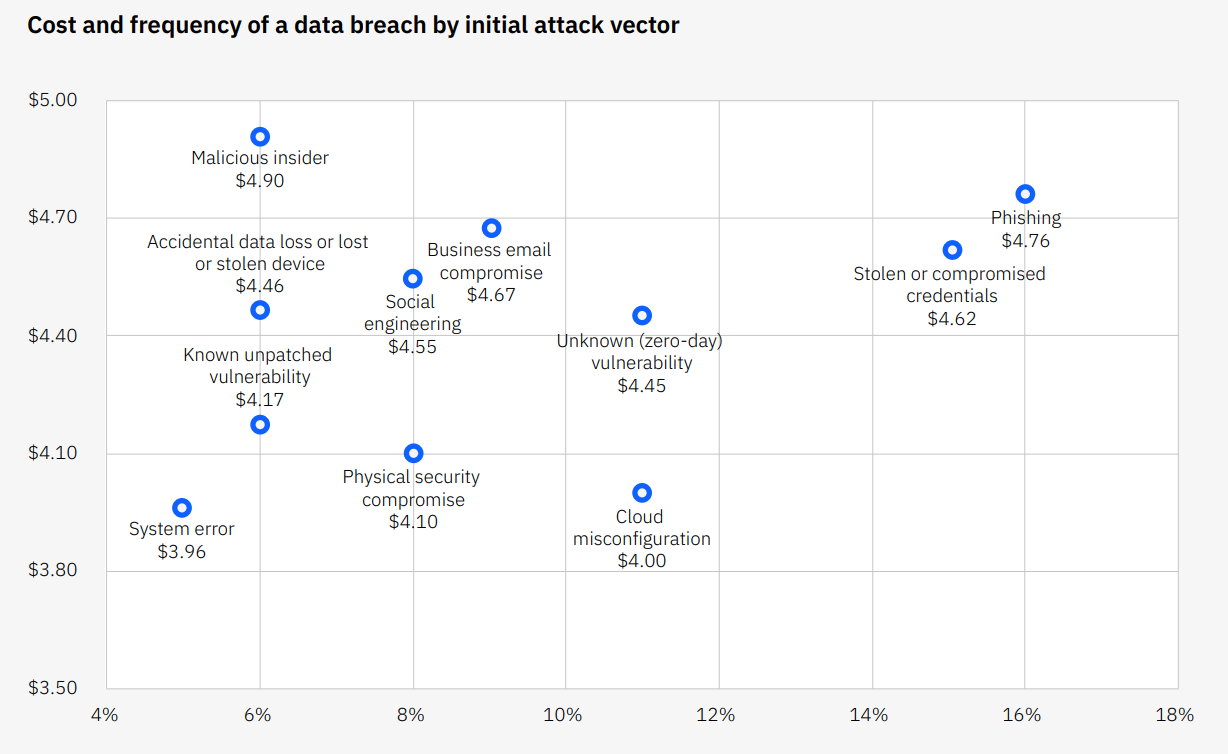
\includegraphics[width=\textwidth]{IBM_Data.Breach.Report.png}
    \caption{Die durchschnittlichen Kosten und Häufigkeiten von Data Breaches, geordnet nach ihrem initialen Angriffsvektor und gemessen in Millionen US-Dollar (2023)\bcite{6_ibmsecurity}.}
\end{figure}
\FloatBarrier

Der obigen Abbildung zufolge richtet ein Data Breach im Durchschnitt 4.45 Millionen US-Dollar an Schaden an, wobei Social Engineering als initialer Angriffsvektor mit 4.55 Millionen US-Dollar noch
über diesem Wert liegt \bcite{6_ibmsecurity}.
Es ist zu beachten, dass initiale Angriffsvektoren wie Phishing oder BEC ebenfalls unter Social Engineering verzeichnet werden könnten und damit den durchschnittlichen finanziellen Schaden weiter steigern würden. \\
Cybercrime hat 2015 einen globalen Schaden von 3 Billionen US-Dollar angerichtet, was sich bis 2021 auf 6 Billionen verdoppelt hat.
Bis 2025 wird prognostiziert, dass sich der weltweite Schaden auf etwa 10.5 Billionen US-Dollar beläuft \bcite{cyberventures}.

Der Verlust nach erfolgreichen Social Engineering Angriffen ist jedoch für Unternehmen weitreichender.
Neben dem direkten finanziellen Verlust durch den Diebstahl der Angreifer erleiden Unternehmen zusätzlich
Wiederherstellungskosten, da etwaige Daten verloren gegangen sind und Sicherheitslücken gefunden und repariert
werden müssen. Des Weiteren entsteht eine Betriebsdisruption, was zu indirektem finanziellen Schaden durch
Verlust von Produktivität führt. Zuletzt erleiden Unternehmen einen Reputationsschaden, was in vielen Fällen
den verheerendsten Faktor ausmacht, insbesondere für kleinere Firmen \bcite{agony}.
Zudem können Unternehmen rechtliche Konsequenzen haben, durch etwaige Haftungsklagen von Kunden oder Behörden, insofern Daten unausreichend gesichert waren.
Sollte der Angriff durch Industriespionage motiviert sein, erleiden Unternehmen zusätzlich einen Verlust von Wettbewerbsvorteilen beziehungsweise einen kompetitiven Schaden in der Marktwirtschaft, da zum Beispiel Geschäftsgeheimnisse gestohlen werden konnten \bcite{kotz}.

Individuen erleiden ebenfalls neben finanziellen- auch weitere Formen von Schäden.
Nicht außer Acht zu lassen ist der emotionale Schaden, da Personen oft in Folge einer erfolgreichen Manipulation als naiv dargestellt werden \bcite{10_bka}.
Reputationsschaden ist ebenfalls ein Faktor, der für Individuen beispielsweise bei Sextortion relevant ist.
\qq{Scham oder die Angst vor Reputationsverlust kann die Anzeigebereitschaft hemmen}\bcite{10_bka}, weshalb ein Social Engineering Angriff eine hohe durchschnittliche Zeit hat, um überhaupt identifiziert zu werden (MTTI\footnote{Mean Time to Identify}).
Der MTTI von Social Engineering liegt bei 218 Tagen, insofern er überhaupt entdeckt wird. Zusammen mit der durchschnittlichen Zeit von etwa 80 Tagen einen Angriff einzudämmen (MTTC\footnote{Mean Time to Contain}), vergehen ungefähr 300 Tage, bis ein Data Breach behoben wird \bcite{6_ibmsecurity}.

\chapter{Psychologie}
\label{chapter:psychologie}

Im Social Engineering werden verschiedene menschliche Eigenschaften ausgenutzt, um eine Person zu manipulieren.
Das Bundeskriminalamt (BKA) hat 2015 in einer Studie \qq{6 soziale Einfallstore [\dots] identifiziert: \begin{itemize}
    \setlength\itemsep{-1em}
    \item Hilfsbereitschaft
    \item Leichtgläubigkeit
    \item Neugier
    \item (Wunsch nach) Anerkennung
    \item Druck
    \item Angst.
\end{itemize}}\bcite{10_bka}

Selbiger Studie ist zu entnehmen, warum die sozialen Angriffsvektoren eine hohe Wirksamkeit erreichen, denn der Begriff selbst
ist Vielen unbekannt und wird sogar oftmals fälschlicherweise mit positiven Assoziationen verbunden.
% \qq{Es gibt keinen Abwehrzauber gegen Social-Engineering, denn dabei handelt es sich um Verhalten,
% das in der Regel sozial erwünscht ist. Technische
% Maßnahmen sind nicht in der Lage, derartige Vorfälle zu verhindern, da es
% sich um ein soziales Problem handelt. Zur Abwehr wird die Fähigkeit benötigt,
% soziale Beziehungen und Kontexte zu deuten.}\bcite{10_bka}
Das bedeutet, dass durch fehlende Aufklärung Opfer nicht das nötige Bewusstsein haben, um eine Situation akurat als Bedrohung zu identifizieren.
Des Weiteren werden beim Social Engineering Verhaltensweisen ausgenutzt, die in der Regel sozial erwünscht sind, weswegen gegen diese nicht vorgegangen werden kann \bcite{10_bka}.


% "Prognostisch bleibt zu befürchten, dass SE-Fälle in Zukunft eher ansteigen als abnehmen
% werden und die Aufklärung problematisch bleibt. Gründe hierfür sind insbesondere:

% Die Betrügereien werden weiterhin und zunehmend aus dem Ausland oder von nicht
% zu identifizierenden Rechnern oder Personen begangen. Dadurch sinkt das Entdeckungsrisiko.
% Scham oder die Angst vor Reputationsverlust kann die Anzeigebereitschaft hemmen.
% Die Aussicht auf immense (schwer abzuschöpfende) Gewinne erhöht den Tatanreiz.
% Die Verfügbarkeit relevanter offener Informationen, die für einen SE-Angriff genutzt
% werden können, wird eher ansteigen als abnehmen. Dadurch werden Manipulationen
% erleichtert.
% Der Druck auf einzelne Mitarbeiter in der heutigen Arbeitswelt steigt eher als dass er
% sinkt und der notwendige Rückhalt/ das Vertrauen in die Organisation, sich vermeintlichen Anweisungen zunächst zu widersetzen, ist nicht immer vorhanden.
% Die "Europäisierung des Betruges" wir nicht adäquat mit der Europäisierung der
% Strafverfolgung beantwortet und "die internationale Rechtshilfe ist in hohem Maße defizitär"."\cite{10_bka}


\section{menschliche Beeinflussung}

\subsection{Einflussprinzipien}

Ein Angreifer kann die Entscheidungsfähigkeit zu seinem Vorteil beeinflussen, denn Menschen reagieren oftmals mit automatisiertem Sozialverhalten \bcite{10_bka}.
Der Psychologe Robert Cialdini entwickelte die sechs Prinzipien der Überzeugung/Beeinflussung (\qq{Six Principles of Persuasion}),
welche in weitreichenden Studien demonstiert wurden\footnote{Da in der Psychologie Situationsfaktoren und menschliche Emotionen immer eine Rolle spielen, ist der Erfolg bei Anwendung dieser Prinzipien nicht garantiert.}\bcite{7_mdpi,psyexploiting}.
Die sechs Prinzipien bestehen aus:

\subsubsection{Authority}
Die meisten Menschen neigen dazu, Autoritätspersonen, beziehungsweise Personen, mit Fachwissen oder ergiebigen Erfahrungen, zu glauben, und gehorchen den Anweisungen eben jener.
Autorität (engl. \qqq{Authority}) kann Menschen selbst dazu verleiten, gegen ihren Glauben oder ihre moralische Vorstellung zu handeln.
Eine Person gilt als Autoritätssymbol, wenn sie als legitimer Experte wahrgenommen wird. Symbole der Autorität, wie etwa Titel, äu\ss eres Erscheinungsbild oder Statussymbole, wie
luxuriöse Gegenstände, erhöhen die Gefolgsamkeit bei Anderen \bcite{7_mdpi,psyprinciples,10_bka}.

\subsubsection{Commitment \& Consistency}
Konsistenz (engl. \qqq{Consistency}) sorgt dafür, dass Personen sich konsequent zu ihren Verpflichtungen (engl. \qqq{Commitments}) und Überzeugungen verhalten.
Das menschliche Verlangen nach Konsistenz gegenüber eingegangenen Verpflichtungen kann das Verhalten einer Person langzeitlich beeinflussen.
Beispielsweise lässt sich dieses Verhalten insofern feststellen, dass Personen die eine kleine Petition unterschreiben später wesentlich gewillter sind, sich auch anderweitig zu diesem Zweck zu engagieren \bcite{7_mdpi,psyprinciples,10_bka}.

\subsubsection{Reciprocity}
Das Prinzip der Gegenseitigkeit (engl \qqq{Reciprocity}) beruht auf der fundamentalen Tendenz, dass sich Menschen dazu verpflichtet fühlen, Gefallen oder Geschenke zu erwiedern.
Dieses Prinzip ist derartig stark, dass die Erwiederung vehementer ausfallen kann, als den initial erhaltenen Gefallen \bcite{7_mdpi,psyprinciples,10_bka}.

\subsubsection{Liking}
Aufgrund des grundlegenden Motivs, soziale Beziehungen aufzubauen und aufrechtzuhalten, führen Menschen die Anfragen Anderer eher aus, wenn sie diese Person kennen oder mögen (engl. \qqq{like}).
Wahrgenommene Ähnlichkeiten erhöhen die Fügsamkeit einer Person. Diese können durchaus oberflächlicher Natur sein, wie etwa ein gemeinsamer Geburtstag oder Name.
Andere Faktoren, die dazu beitragen von einer Person gemocht zu werden, sind physische Attraktivität und positive Assoziation, etwa durch Komplimente \bcite{7_mdpi,psyprinciples,10_bka}.

\subsubsection{Social Proof}
Das Prinzip des sozialen Beweises (engl. \qqq{social proof}) ist ein Phänomen, dass in der Psychologie als \qqq{informativer sozialer Einfluss} bekannt ist.
Es geht um eine mächtige Überzeugungstaktik, die ausnutzt, dass Menschen eine natürliche (bzw. primitive) Tendenz haben, dem Beispiel Anderer folgen zu wollen, um sozial akzeptiert zu werden \bcite{7_mdpi,psyprinciples,10_bka}.

\subsubsection{Scarcity}
Das letzte Prinzip der Überzeugung ist die Knappheit (engl. \qqq{scarcity}), und beschreibt die Tatsache, dass Menschen einer geringeneren Quantität eine höhere Qualität zuschreiben.
Dieses Prinzip ist nicht ausschließlich auf Materielles anzuwenden, sondern gilt beispielsweise auch bei verhaltenstechnisch weniger verfügbaren Möglichkeiten, oder bei Informationen, die nicht allgemein erhältlich sind.
So wirken Informationen, die einem im Geheimen anvertraut werden, oft spektakulärer \bcite{7_mdpi,psyprinciples,10_bka}.

\subsection{Persönlichkeitsmerkmale}

Das Fünf-Faktor-Modell ist ein Modell der Persönlichkeitspsychologie, welches fünf Kernaspekte der Persönlichkeit identifiziert und besagt, dass jeder Mensch sich auf den Skalen dieser Kernaspekte einordnen lässt.
Die fünf Eigenschaften bieten also jeweilige Skalen im Wertebereich von 0 bis 100.
Das Modell wird auch als OCEAN-Modell bezeichnet (nach den entsprechenden Anfangsbuchstaben Openness, Conscientiousness, Extraversion, Agreeableness, Neuroticism\footnote{zu Deutsch: Offenheit, Gewissenhaftigkeit, Extraversion, Verträglichkeit, Neurotizismus}).
Die folgende Tabelle beschreibt knapp die verschiedenen Kerneigenschaften:

\begin{table}[!htp]
    \centering
    \begin{tabular}{ |c|m{11em}|m{11em}| }
        \hline
        \textbf{Eigenschaft} & \textbf{hoher Wert}                                                      & \textbf{niedriger Wert}                                   \\
        \hline \hline
        Offenheit            & intellektuell, fantasievoll, kontaktfreudik. Offen für Neues             & praktisch, konventoniell, skeptisch, rational             \\
        \hline
        Gewissenhaftigkeit   & organisiert, eigenständig, gründlich, zuverlässig, aber kontrollierend   & desorganisiert, nachlässig, kann anfällig für Sucht sein  \\
        \hline
        Extraversion         & aufgeschlossen, enthusiastisch, aktiv; sucht Neues                       & distanziert, ruhig, unabhängig; vorsichtig, zurückgezogen \\
        \hline
        Verträglichkeit      & vertrauensvoll, unkompliziert, empathisch, nachgiebig, umgänglich        & unkooperativ, feindselig; unempathisch                    \\
        \hline
        Neurotizismus        & anfällig für Stress, Angst, Befangenheit, Launenhaftigkeit, Impulsivität & emotional stabil, ruhig und sicher.                       \\
        \hline
    \end{tabular}
    \caption{Charakteristiken der OCEAN-Modell Persönlichkeitseigenschaften, entnommen aus \bcite{psyse}.}
\end{table}
\FloatBarrier

\subsection{Anfälligkeit für Social Engineering}

Gewisse Persönlichkeitseigenschaften sind direkt korreliert mit der Anfälligkeit verschiedener Prinzipien der Beeinflussung, und damit dem Social Engineering.
Es gibt drei verschiedene Persönlichkeitsmodelle im Zusammenhang mit Social Engineering: FFM (Five-Factor Model), MBTI (Myers-Briggs Type Indicator), DT (Dark Triad Model).
Die folgende Grafik verdeutlicht den Zusammenhang zwischen bestimmten Überzeugungsprinzipien und Persönlichkeitsmerkmalen, von denen aus psychologischer Sicht ausgegangen wird, nach dem FFM Modell:

\begin{figure}[!htp]
    \centering
    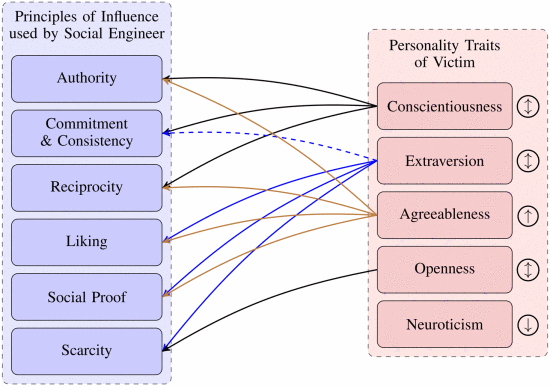
\includegraphics[scale=.55]{FFM.png}
    \caption{Anfälligkeit verschiedener Persönlichkeitseigenschaften durch die Prinzipien der Beeinflussung, welche von Social Engineers verwendet werden (Die Färbung der Pfeile ist außer Acht zu lassen; Gestrichelte Linien weisen auf eine negative Korrelation hin). Entnommen aus \bcite{7_mdpi}.}
\end{figure}
\FloatBarrier

Gewissenhaftigkeit erhöht die Empfänglichkeit für Autorität, Engagement/Konsistenz und Reziprozität.
Extraversion erhöht die Empfänglichkeit für Sympathie und soziale Anerkennung (soziale Beweise) aufgrund ihrer Verbindung mit Geselligkeit.
Hohe Grade der Verträglichkeit korrelieren mit der Tendenz, anderen zu vertrauen und erhöhen die Anfälligkeit für Social Engineering, da sie anfälliger für Überzeugung und Autorität sind,
und mehr Interesse an sozialer Bestätigung, Reziprozität und Sympathie haben.
Offenheit ist mit erhöhter Anfälligkeit für Social-Engineering-Taktiken verbunden, da sie mit der sozialen Neigung einhergeht, Neues erleben zu wollen.
Neurotizismus ist mit Stress und Angst verbunden, was wiederum die Anfälligkeit gegebenenfalls verringern kann \bcite{psyexploiting,7_mdpi}.

Nach dem DT-Modell haben narzistische (oder psychopathische) Tendenzen eine Korrelation dazu, den Angreifer einer Social Engineering Attacke zu repräsentieren.
Narzismus zeichnet sich zumeist aus durch hohe Extraversion und hohen Neurotizismus, sowie niedrige Verträglichkeit \bcite{psyexploiting}.

Insgesamt ist also zu sehen, dass nahezu alle Persönlichkeiten auf gewisse Manipulationstechniken ansprechen.
Daher ist also auch nahezu jede Person, bei Verwendung eines spezifischen und passenden Prinzips der Beeinflussung, manipulierbar.

\chapter{Prognose}

prognose hier ...



\phantomsection
\addcontentsline{toc}{bibliography}{\bibname}
\bibliographystyle{plain}
\bibliography{references}

\end{document}